\section{Multicore Systeme}

\subsection{Geschwindigkeit auf Prozessor steigern}

\subsubsection{Clockfrequenz erhöhen}

\begin{outline}
    \1 PCB-Design wird sehr anspruchsvoll (Leistungslängen, Reflexionen, etc.)
    \1 Elektrinsche Verlustleistung steigt \textbf{linear} mit Clockfrequenz: $P = f_{\rm cl} \cdot C_L \cdot V_{\rm dd}^2$
    \1 Lichtgeschwindigkeit ist Grenze (Licht legt in $1 \, \nano \second$ $30 \, \centi \meter$ zurück)
\end{outline}

\vspace{0.1cm}

\textrightarrow\ Erhöhung der Clockfrequenz hat eigentlich nur Nachteile


\subsubsection{Instruction-level parallelism (ILP)}

\begin{outline}
    \1 Parallelismus wird auf \textbf{Instruktionslevel} angestrebt
        \2 Pipelines
        \2 Verschachteln der Instruktionen, um Pipeline möglichst optimal auszulasten
        \2 Vermeiden von Pipline flush durch Vorhersage der Verzweigung (branch prediction)
    \1[-] Branch prediction kann sehr aufwendig werden
    \1[-] Compiler werden komplex
\end{outline}


\subsubsection{Thread-level parallelism (TLP)}

\begin{outline}
    \1 Parallelisierte Einheit ist in der Grössenordnung einer Funktion
        \2 Umfangreichere Stufe der Parallelisierung
    \1 Zugriffe auf gemeinsame Ressourcen (z.B. shared memory) müssen geregelt sein
    \1 Design Issues
        \2 Jeder Thread erzeugt Overhead (Stack, context switch bei single-core Prozessor)
        \2 Nicht beliebig viele Threads möglich
        \2 Bei zu vielen Threads (wenn zusammengehöriges auseinandergenommen wird), dann werden
            gewisse Daten unnötigerweise shared
\end{outline}


\para{Umsetzung von TLP auf Uniprozessor (single-core)}

\begin{outline}
    \1 Threads werden time-sliced
    \1 Pseudo-TLP
    \1 Context switch notwendig (Umschalten von einem zum anderen Thread)
    \1 \textbf{Ergibt keinen Geschwindigkeitsgewinn}
\end{outline}


\para{Umsetzung von TLP auf Multiprozessor}

\begin{outline}
    \1 Mehrere parallele Prozesse können je einen Thread bearbeiten
    \1 Echter-TLP
    \1 Clockfrequenz kann tiefer gehalten werden
    \1 Einfache Hardware wird multipliziert
    \1 Datenaustausch zwischen Prozessen muss geregelt werden, z.B. mit Message Passing / Shared Memory
\end{outline}


\subsection{Speicherorganisation auf Multicore Prozessor}

\begin{minipage}[t]{0.45\columnwidth}
    \raggedright
    \para{Shared Memory}

    \begin{outline}
        \1 Alle Prozessoren nutzen einen gemeinsamen Speicher
            \2 Kann zum Falschenhals werden
    \end{outline}
\end{minipage}
\hfill
\begin{minipage}[t]{0.53\columnwidth}
    \raggedright
    \para{Distributed Memory}

    \begin{outline}
        \1 Jeder Prozessor hat eigenen lokalen Speicher
            \2 Braucht Mechanismus für Datenaustausch, z.B. Message Parsing
    \end{outline}
\end{minipage}


\subsubsection{Multicore Prozessor}

\begin{outline}
    \1 Speizieller Multiprozessor \textrightarrow\ alle Cores (Prozessoren) auf demselben Chip
    \1 MIMD (Multiple Instructions Multiple Data)
    \1 Komplexe Speicherorganisation
        \2 Caches, per core local memory, Shared Memory
    \1 Homogene vs. heterogene Multicore Prozessoren
\end{outline}


\subsubsection{Embedded Computing vs. PC/Enterprise Computing}


\para{PC / Enterprise Computing}

\begin{outline}
    \1 Meist \textbf{homogene} Multicores
        \2 Gesamtaufgabe aufteilen für optimale Ausühtungszeit \textrightarrow\ Amdahl's Law
    \1 Parallelisierung möglichst automatisiert (z.B. durch Compiler)
\end{outline}

\para{Embedded Computing}

\begin{outline}
    \1 Oft \textbf{heterogene} Multicores
        \2 ARM Core für administrative Aufgaben
        \2 ein bis mehrere DSPs für effiziente mathematische Berechnungen
        \2 Aufteilung ergibt sich von selbst
\end{outline}


\subsection{Amdahl's Law}

Amdahl's Law beschreibt den theoretisch mögichen Speedup $S$ eines parallellen Tasks, wenn dieser
auf mehrere Cores (Prozessoren) aufgeteilt wird. \\
\textbf{Hinweis:} Typischerweise bleibt ein Teil des Tasks sequenzell. Dieser kann nicht aufgeteilt werden
und \textbf{limitiert} somit den möglichen Speedup.

\vspace{0.1cm}

% \begin{minipage}[t]{0.48\columnwidth}
%     $$ S(n) = \frac{1}{1 - p + \frac{p}{n}} $$
%     $$ S \leq \frac{1}{1-p} $$
        
%     \begin{tabular}{ll}
%         $S$     & Speedup (Faktor, z.B. 4.0)            \\
%         $p$     & Parallel Portion (z.B. 0.5 = 60 \%)   \\
%         $n$     & Anzahl Cores                  
%     \end{tabular}
% \end{minipage}
% \hfill
% \begin{minipage}[t]{0.48\columnwidth}
%     $$ S(n) = \frac{T}{t_s + \frac{t_p}{n}} $$
%     $$ S \leq \frac{T}{T - t_p} = \frac{T}{t_s} $$

%     \begin{tabular}{ll }
%         $T$     & Totale Ausführungszeit        \\
%         $t_p$   & Parallele Ausführungszeit     \\
%         $t_s$   & Serielle Ausführungszeit  
%     \end{tabular}
% \end{minipage}

\begin{minipage}[c]{0.25\columnwidth}
    $$ S(n) = \frac{1}{1 - p + \frac{p}{n}} $$
    $$ S \leq \frac{1}{1-p} $$
\end{minipage}
\hfill
\begin{minipage}[c]{0.25\columnwidth}
    $$ S(n) = \frac{T}{t_s + \frac{t_p}{n}} $$
    $$ S \leq \frac{T}{T - t_p} = \frac{T}{t_s} $$
\end{minipage}
\hfill
\begin{minipage}[c]{0.48\columnwidth}
    \begin{tabular}{ll}
        $S$     & Speedup (Faktor, z.B. 4.0)            \\
        $p$     & Parallel Portion (z.B. 0.6 = 60 \%)   \\
        $n$     & Anzahl Cores                          \\
        $T$     & Totale Ausführungszeit                \\
        $t_p$   & Parallele Ausführungszeit             \\
        $t_s$   & Serielle Ausführungszeit  
    \end{tabular}
\end{minipage}


\subsection{Memory Hierarchy}

\begin{center}
    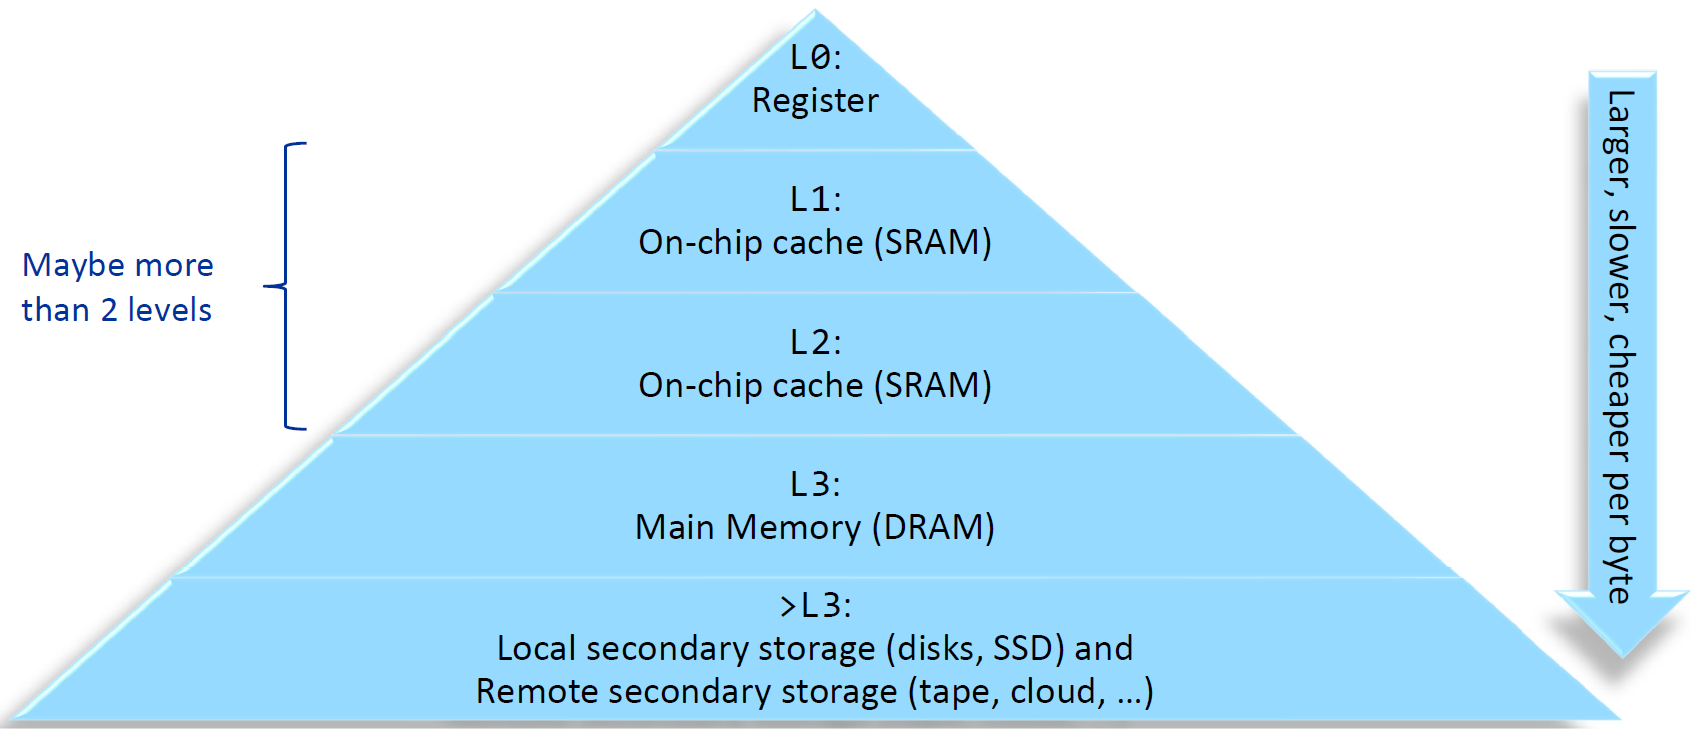
\includegraphics[width=0.88\columnwidth]{images/multiprocessor_memory.png}
\end{center}


\subsection{Cache-Speicher}

\begin{outline}
    \1 Für Prozessor versteckte, schnelle Speicher \textrightarrow\ liegen zw. Prozessor und Hauptspeicher
    \1 \textbf{Führen Kopie von häufig benötigten Hauptspeicherdaten}
        \2 Nutzen zeitliche und örtliche Lokalität von Programmen aus
    \1 \textbf{Cache Hit:} Vom Prozessor benötigte Hauptspeicherdaten sind im Cache
        \2 Schnellerer Zugriff möglich
    \1 \textbf{Cache Miss:} Daten müssen aus Hauptspeicher geholt werden
 \end{outline}

 $$ \boxed{ \text{Mittlere Zuegriffszeit} = (\text{Hit Time}) \cdot (\text{Hit Rate}) + (\text{Miss Penalty}) \cdot (\text{Miss Rate}) } $$


 \begin{tabular}{l c l}
    (Hit Time)      & $=$   & (Zeit zur Bestimmung von Hit oder Miss) $+$   \\
                    &       & (Speicherzugriffszeit auf Cache)              \\
    (Miss Penalty)  & $=$   & (Zeit zur Bestimmung von Hit oder Miss) $+$   \\
                    &       & (Zeit zum Ansprechen der nächsten Ebene) $+$  \\
                    &       & (Zeit zum Übertragen von der nächsten Ebene)
 \end{tabular}      


\subsubsection{Zeitliche / örtliche Lokalität}

\para{Zeitliche Lokalität (Temporal locality)}

\begin{outline}
    \1 Soeben verwendete Daten / Instruktionen werden mit hoher \myul{Wahrscheinlichkeit} bald wieder verwendet
        \2 \textbf{Caches nutzen zeitliche Lokalität aus}
\end{outline}


\para{Örtliche Lokalität (Spatial locality)}

\begin{outline}
    \1 Bei soeben verwendete Daten / Instruktionen werden mit hoher \myul{Wahrscheinlichkeit} auch benachbarte Daten / Instruktionen verwendet
        \2 Caches: Wenn auf eine bestimmte Adresse das erste Mal zugegriffen wird, werden nicht nur die Daten von dieser Adresse ins Cache 
            geladen, sondern ein Speicherblock bestimmter Grösse um diese Adresse herum
\end{outline}

\vspace{0.1cm}

\textrightarrow\ Cache ist reine Wahrscheinlichkeit! \textrightarrow\ Hoffen, dass Daten dort sind...

